\documentclass[3p]{elsarticle} %review=doublespace preprint=single 5p=2 column
%%% Begin My package additions %%%%%%%%%%%%%%%%%%%
\usepackage[hyphens]{url}



\usepackage{lineno} % add
\providecommand{\tightlist}{%
  \setlength{\itemsep}{0pt}\setlength{\parskip}{0pt}}

\bibliographystyle{elsarticle-harv}
\biboptions{sort&compress} % For natbib
\usepackage{graphicx}
\usepackage{booktabs} % book-quality tables
%%%%%%%%%%%%%%%% end my additions to header

\usepackage[T1]{fontenc}
\usepackage{lmodern}
\usepackage{amssymb,amsmath}
\usepackage{ifxetex,ifluatex}
\usepackage{fixltx2e} % provides \textsubscript
% use upquote if available, for straight quotes in verbatim environments
\IfFileExists{upquote.sty}{\usepackage{upquote}}{}
\ifnum 0\ifxetex 1\fi\ifluatex 1\fi=0 % if pdftex
  \usepackage[utf8]{inputenc}
\else % if luatex or xelatex
  \usepackage{fontspec}
  \ifxetex
    \usepackage{xltxtra,xunicode}
  \fi
  \defaultfontfeatures{Mapping=tex-text,Scale=MatchLowercase}
  \newcommand{\euro}{€}
\fi
% use microtype if available
\IfFileExists{microtype.sty}{\usepackage{microtype}}{}
\usepackage{graphicx}
% We will generate all images so they have a width \maxwidth. This means
% that they will get their normal width if they fit onto the page, but
% are scaled down if they would overflow the margins.
\makeatletter
\def\maxwidth{\ifdim\Gin@nat@width>\linewidth\linewidth
\else\Gin@nat@width\fi}
\makeatother
\let\Oldincludegraphics\includegraphics
\renewcommand{\includegraphics}[1]{\Oldincludegraphics[width=\maxwidth]{#1}}
\ifxetex
  \usepackage[setpagesize=false, % page size defined by xetex
              unicode=false, % unicode breaks when used with xetex
              xetex]{hyperref}
\else
  \usepackage[unicode=true]{hyperref}
\fi
\hypersetup{breaklinks=true,
            bookmarks=true,
            pdfauthor={},
            pdftitle={The importance of measurement uncertainty in ecological management},
            colorlinks=true,
            urlcolor=blue,
            linkcolor=magenta,
            pdfborder={0 0 0}}
\urlstyle{same}  % don't use monospace font for urls

\setcounter{secnumdepth}{0}
% Pandoc toggle for numbering sections (defaults to be off)
\setcounter{secnumdepth}{0}
% Pandoc header
\journal{The American Naturalist} \usepackage{lineno} \linenumbers
\modulolinenumbers[3]
\usepackage{setspace} \doublespacing



\begin{document}
\begin{frontmatter}

  \title{The importance of measurement uncertainty in ecological management}
    \author[]{Authors removed during peer review}
  
  
    
  \begin{abstract}
  Ecological management and decision-making typically focus on uncertainty
  about the future, but surprisingly little is known about how to account
  for uncertainty of the present: that is, the realities of having only
  partial or imperfect measurements. Our two primary paradigms for
  handling decisions under uncertainty -- the precautionary principle and
  optimal control -- have so far given entirely controdictory results.
  This paradox is best illustrated in the example of fisheries management,
  where many ideas that guide our thinking about ecological decision
  making were first developed. There, we find that simplistic optimal
  control approaches have repeatedly concluded that a manager should
  increase catch quotas when faced with greater uncertainty about the
  standing stock biomass. Meanwhile, most current best practices take a
  more precautionary approach, decreasing catch quotas by a fixed amount
  to account for uncertainty. Using comparisons to both simulated and
  historical catch data, we find that neither approach is sufficient to
  avoid stock collapses under moderate observational uncertainty. Using
  cutting-edge point-based partially observed Markov decision process
  (POMDP) methods, we demonstrate how this paradox arises from flaws in
  the standard management theory, which contributes to over-exploitation
  of fisheries and increased probability of economic and ecological
  collapse. In contrast, we find POMDP-based management avoids such
  over-exploitation while also generating higher economic value through
  adaptive learning. These results have significant implications for how
  we handle uncertainty in both fisheries and ecological management more
  generally. Dealing with uncertainty in decisions requires approaches
  which are both adaptive and explicit about uncertainty, such as POMDPs.
  \end{abstract}
   \begin{keyword} Measurement uncertainty \sep POMDP \sep Decision theory \sep Fisheries \sep Conservation \sep \end{keyword}
 \end{frontmatter}

Imperfect information is ubiquitous in ecological management and
conservation decision making. While the pressing concerns of global
change have put the spotlight on \emph{forecasting}, i.e.~the
uncertainty of the future (e.g. Petchey et al. 2015), management
decisions must also contend with uncertainty of the \emph{present}: How
many fish are in the sea today? What regions harbor the most fragile
biodiversity? How have invasive species transformed native communities?
A recognition of the importance of uncertainty as well as sophisticated
methods and tools to do so has become increasingly widespread in the
context of estimating ecological models from available data, thanks in
large part to the rise of approaches such as Hierarchical Bayesian
Modeling, along with convenient software tools for implementing these
methods. In sharp contrast to that shift, the treatment of uncertainty
in decisions -- how the uncertainty in models should be reflected in
scientific recommendations, remains far less developed, more
qualitative, and under-served by available tools. In this paper we
illustrate how uncertainty in measurement has a dramatic negative impact
on outcomes under a variety of these existing approaches, which can be
avoided through the use of more formal approaches that have since been
developed in other fields that can likewise be implemented in software
tools. This insight both resolves a long-standing paradox in fisheries
management and has important implications for how ecosystem management
deals with uncertainty more generally.

Approaches for decision making under uncertainty in ecological systems
can be divided into two camps: approaches based in ``optimal control''
and usually favored by natural resource economists, and approaches based
in heuristic methods such as scenario planning, resilience thinking, and
precautionary rules of thumb, more commonly found in both ecological
literature and actual practice (Fischer et al. 2009; Polasky et al.
2011). While researchers have for some time recognized the need to unify
the transparent and quantitative algorithmic approach of optimal control
with the greater complexity and uncertainty of real ecosystems that is
acknowledged by heuristic methods, computational barriers to doing so
have hither-to stymied this progress. Here, we illustrate how the
limitations of these approaches has been manifested in the example of
fisheries management, and present a new approach that can combine the
reality of measurement uncertainty and the rigor of optimization to
resolve a long-standing paradox and suggest a more robust approach to
management.

Fisheries conservation and management has long been both a crucible and
proving ground for the theory of ecological management more generally,
including topics such as adaptive management (Walters and Hilborn 1978),
ecosystem-based management (Levin and Lubchenco 2008) and resilience
thinking (Holling 1973; May 1977), while also giving rise to the
sub-discipline of resource economics (Gordon and Press 1954; Schaefer
1954; Beverton and Holt 1957), thanks to its global relevance, long
history, and readily available data. Consequently, understanding the
impact of measurement uncertainty in this rich and well-studied context
will have implications for both resource management and conservation
efforts in other domains, many of which draw on concepts established or
tested in fisheries ecosystems. In particular, the approach here
illustrates the limitations of both over-simple optimal control
approaches and rule-of-thumb precautionary approaches, and offers
instead a more general strategy for dealing with measurement uncertainty
adaptively.

We compare the results of managing simulated fish stocks under the
existing optimal control approach, a heuristic approach that more
closely resembles today's management practices, and a newly proposed
approach that provides a more rigorous treatment of uncertainty.

\section{The Decision Problem}\label{the-decision-problem}

We consider the management problem of setting catch quotas for a marine
fishery in the face of imperfect information about the current stock
size and uncertainty about future recruitment.

We seek to determine the sequence of actions \(h_t\) for
\(t \in [1, ... \infty]\) that maximize the net present value
(discounted sum of all future profits) of the fishery. We will denote
the discount rate \(\gamma\). For simplicity we will once again follow
classic theory and assume a fixed price for fish, (equivalently,
measuring our value in units of discounted fish rather than discounted
dollars), though again this assumption is easy to relax. Each year, the
manager also obtains an estimate \(y_t\) of the true \(x_t\) stock size
subject to some measurement uncertainty \(\xi_t\)

\[y_t = \xi_t x_t\]

For simplicity we will assume measurement uncertainty is normally
distributed with standard deviation \(\sigma_m\),
\(\xi \sim \mathcal{N}(1, \sigma_m)\). Given an estimated recruitment
model along with this measurement of the stock size, the manager must
choose the set of a harvest quotas \(\lbrace h_t \rbrace\) for
\(t \in [0, 1, \infty]\) that maximizes expected long term (net) present
value:

\[\max_{ \lbrace h_t \rbrace } \mathbb{E} \left \{ \sum_{t=0}^{\infty} \gamma^t \cdot h_t \right \}\]

A few subtleties arise in this seemingly simple problem statement that
we must address. First, given our discrete-time formulation of the
recruitment process, it is necessary to decide if the measurement
\(y_t\) happens before or after harvest \(h_t\): that is do we: measure,
recruit, harvest, or measure, harvest, recruit? Following convention in
the optimal control literature (e.g. (Reed 1979; Clark 1990; Sethi et
al. 2005)), we will assume the latter; measurement occurs immediately
before harvest, followed by recruitment.

A second subtly is in the nature of the decision problem itself: note
that the manager in not myopic, thinking only about the next year, but
rather considers the sequence of all future actions \({h_t}\). While the
manager will revisit this sequence each year in light of new
observations, it is this ability of the decision problem to think ahead
that allows it to tolerate short-term costs (e.g.~reduced harvests in
the current season) for larger future payoffs. In this, ecological
management is a game of chess, always thinking several moves ahead. This
differs from the problem solved in theory as well as the practice of
maximum sustainable yield, which seeks to identify only a fixed
mortality \(F_{MSY}\) applied for all time, rather than a \emph{policy}
of varying quotas \(h_t\) depending on the stock assessment \(y_t\).
Understanding this distinction is key both to understanding the
differences between current theory and current best practice in
fisheries management.

\subsection{Population model}\label{population-model}

To facilitate tractability and interpretation, we will focus on the
well-studied Gordon-Schaefer model (Gordon and Press 1954; Schaefer
1954) of logistic population growth (stock recruitment),

\[x_{t+1} = \varepsilon_t (x_t-h_t) r  \left(1 - \frac{(x_t-h_t)}{K}\right) \]

where \(x_t\) is the current stock size, \(h_t\) the harvest chosen that
year, with parameters \(r\) giving the individual growth rate, and \(K\)
the carrying capacity and \(\varepsilon\) representing stochastic
recruitment in a variable environment. We have written this in terms of
\(x_t - h_t\) to underscore that we assume the convention of observe,
harvest, recruit. We will assume for simplicity
\(\varepsilon \sim \mathcal{N}(1, \sigma_g)\). This and similar models
are widely used in large scale analyses across diverse stocks (e.g.
(Costello et al. 2016; Britten et al. 2017)), and form the basis for
much of bioeconomic theory (Clark 1990). As such, it will be easier to
compare our results against intuition and classic theory, and avoid the
possibility of differences arsing only because of some particular subtle
assumption hidden in a more complex model.

It is important to remember that both existing methods we discuss and
the POMDP approach proposed here can or are already applied to more
complex models as well, including those with age or stage structure.
Likewise, while we consider the model and it's parameters as ``given,''
it should be understood to mean that this in practice comes as the
result of some model choice and statistical estimation from historical
data, frequently accounting for uncertainty in both the process and the
measurements (e.g. Dichmont et al. 2016). As we shall see here, having
included uncertainty in the model \emph{estimation} in no way excuses us
from having to also deal once again with that uncertainty in the
decision process.

\section{Current Theory and Practice}\label{current-theory-and-practice}

Gordon and Press (1954) and Schaefer (1954) independently showed in the
same year that the maximum sustainable yield for the model bearing their
names is achieved by reducing the stock to the population to the size at
which it obtains the maximum growth rate which is known as Biomass at
Maximum Sustainable Yield, \(B_{MSY}\). For the Gordon-Schaefer model
(and many others), this is achieved at \(B_{MSY} = K/2\). They observed
that fishing at a \emph{constant yield} (that is, an individual fish
mortality, \(F\), such that harvest \(H = F \cdot B\)) of
\(F_{MSY} := \tfrac{H_{MSY}}{B_{MSY}}\)) will eventually lead to a
population that converges to the biomass \(B_{MSY}\) and produces the
maximum sustainable harvest, \(H_{MSY} = r K / 4\) in this model. From
here, theory and practice diverge.

This \emph{constant yield} (constant mortality) solution thus
corresponds to an equilibrium analysis which does not solve the
time-dependent optimization problem above. In particular, this maximum
sustainable yield (MSY) strategy will not be optimal whenever the stock
is away from \(B_{MSY}\). Clark (1973) demonstrated (assuming no
uncertainty in measurement or stochasticity in population dynamics) that
the optimal time-dependent strategy is not one of constant yield, but
rather of \emph{constant escapement}. We will return to this approach in
a moment.

\subsection{Uncertainty in Practice: MSY \&
TAC}\label{uncertainty-in-practice-msy-tac}

Maximum Sustainable Yield (MSY) remains the basis of international law
(including the UN, IWC, IATTC, ICCAT, ICNAF; Mace (2001)) and a familiar
standard of management in terrestrial ecosystems as well as aquatic
(Clark 1990). Critics have for some time observed the limitations of
harvesting at MSY in face of uncertainty in stock sizes and population
dynamics (Larkin 1977; Botsford et al. 1997). Many US fisheries reflect
this uncertainty through a series of adjustments that effectively reduce
the target fishing mortality level to reflect this uncertainty.
Typically, a stock assessment model provides a best estimate of
\(B_{MSY}\) and corresponding mortality \(F_{MSY}\) is used to define
the stock Over-fishing Limit, (OFL). Based on this, a somewhat lower
level is set as the Allowable Biological Catch (ABC), reflecting
uncertainty in the stock assessment. To reflect possible uncertainty
between reported and actual catch, the ABC is reduced somewhat further
to define the Total Allowable Catch, (TAC), which forms the basic unit
of management for many such fisheries. To reflect this process, our
analysis will also consider policies in which the harvest quota is set
at 80\% of the level expected under the MSY policy:
\(H_{TAC}(t) = 0.8 \cdot F_{MSY} \cdot B_t\), for a biomass estimated at
\(B(t)\) in year \(t\). To distinguish this approach from MSY, we will
refer to this approach as a TAC policy. This more closely represents a
heuristic (e.g. Hilborn 2010) or resilience-based approach (sensu
Fischer et al. 2009) than an optimization-based policy. Importantly,
this approach shares the fundamentally stationary assumptions of an MSY
policy by defining a constant mortality rather than a dynamic policy.
Thus, despite being more cautious overall and generating lower economic
yield than a constant escapement policy, TAC policies continue to
harvest at non-zero rates even if a stock falls below \(B_{MSY}\), while
the constant escapement policy does not.

\subsection{Optimal management}\label{optimal-management}

So far, attempts to provide a more formal basis for managing uncertainty
than the heuristic adjustment of catch limits described above have
largely foundered in a series of paradoxes. Without uncertainty, the
theoretical policies are quite intuitive: The result derived by Clark
(1973) for an optimal dynamic strategy to replace the equilibrium
solution of MSY can be summarized as: If the stock is most productive at
\(B_{MSY}\), then obtain \(B_{MSY}\) as quickly as possible. Thus, at
any level below \(B_{MSY}\), the economically optimal thing to do is to
completely shut down the fishery, while above this stock, harvests
greater than \(H_{MSY}\) will be needed to bring the stock back to
\(B_{MSY}\). (This intuition must be adjusted slightly in the case of
economic discounting of future profits, but is otherwise quite general,
see Clark (1990)). This strategy is known as constant escapement, since
a constant sock size \(B_{MSY}\) escapes harvest each year. While both
converge to the same long-term biomass and long-term yield, these
differences away from equilibrium between the mortality-based approach
that dominates fisheries management practice and the escapement-based
approach that became the focus of theory will result in different
behaviors under uncertainty. Intuitively, any uncertainty, either in the
population growth model (stochasticity), or measurement error, should
seem to justify harvesting fewer fish, as is built into the TAC limits
discussed above. Yet formal treatments of these issues have so far
required approximations, and these approximations have driven
paradoxical conclusions which we briefly summarize here.

\subsection{\texorpdfstring{Reed's Paradox:
\(S = D\)}{Reed's Paradox: S = D}}\label{reeds-paradox-s-d}

The first of these we shall refer to as Reed's Paradox for stochastic
growth, owing to the mathematical proof provided in Reed (1979) which
demonstrates that, under sufficiently general assumptions, the optimal
escapement \(S\) for a population under stochastic growth, is identical
to the optimal escapement \(D\) of a deterministic population,
\(S = D = B_{MSY}\). This surprising result suggests that in going from
a world where a manager has perfect knowledge of absolutely everything
into a scenario where the manager faces considerable uncertainty about
the future state of the world, no additional precaution is needed. This
also provides the manager with a remarkably convenient mechanism for
determining the optimal harvest policy: rather than rely on
computationally intensive Stochastic Dynamic Programming to determine
the optimal policy, a simple derivative will suffice, which is all that
is needed to solve the maximum of the deterministic problem.

\subsection{Clark's Paradox}\label{clarks-paradox}

Clark and Kirkwood (1986) was among the first attempts to resolve Reed's
Paradox. Clark and Kirkwood (1986) (quite correctly, as we will see),
identified the crux of Reed's Paradox as the absence of measurement
uncertainty:

\begin{quote}
An important tacit assumption in Reed's analysis, as in the other works
referred to above, is that the recruitment level X is known accurately
prior to the harvest decision, {[}\ldots{}{]} In the case of fishery
resources, the stock level X is almost never known very accurately,
owing to the difficulty of observing fish in their natural environment.
\end{quote}

Unfortunately, Clark and Kirkwood (1986) was unable to solve the
resulting problem exactly, but had to adopt an almost equally
troublesome assumption:

\begin{quote}
For reasons of tractability, we shall adopt the simplifying assumption
that the escapement level S, is known exactly at the end of that period.
(The mathematical difficulty of the problem increases markedly if this
assumption is relaxed.)
\end{quote}

Unfortunately for Clark and Kirkwood (1986), this ``simplifying
assumption'' serves to squash most of the measurement error, and their
results instead only deepened the paradox, finding policies that become
even \emph{less} cautious as uncertainty increases:

\begin{quote}
{[}Our{]} results appear to contradict the conventional wisdom of
renewable resource management, under which high uncertainty would call
for increased caution in the setting of quotas.
\end{quote}

Relying on a quite different but still flawed assumption nearly two
decades later, Sethi et al. (2005) largely confirm Clark's Paradox,
which they likewise observed with some concern:

\begin{quote}
It may seem counter-intuitive that a measurement error causes lower
expected escapements below the deterministic fishery closure threshold.
\end{quote}

Despite these notes of caution, both Clark and Kirkwood (1986) and Sethi
et al. (2005) ultimately attempt to rationalize this counter-intuitive
conclusion rather than reject it. Others have also attempted to
introduce measurement error, but always relying on various
approximations that similarly alter the problem. The most common such
assumption is to assume from the outset that the solution must be of
`constant-escapement' type (Ludwig and Walters 1981; Roughgarden and
Smith 1996; Engen et al. 1997; Moxnes 2003). Here we will illustrate the
use of powerful modern algorithms that will permit a more direct
solution to the case of measurement uncertainty. In addition to
resolving this paradox, we will demonstrate this direct solution also
out-performs current more heuristic rules of thumb such as those
currently used in fisheries management to account for uncertainty.

\subsection{POMDPs: An optimal treatment of measurement
uncertainty}\label{pomdps-an-optimal-treatment-of-measurement-uncertainty}

As discussed above, absent the short-cut provided by Reed's theorems --
solving for the optimal management policy in a stochastically
fluctuating population -- involves a Markov Decision Process (MDP),
commonly referred to in ecological literature by its solution method,
Stochastic Dynamic Programming (SDP). The constant escapement (CE)
strategy considered here is the result of such an MDP or SDP analysis.
Once measurement uncertainty is introduced, the problem becomes a
Partially Observed Markov Decision Process (POMDP, not be confused with
a partially observed or hidden Markov model, HMM, in which no decision
process is involved). The POMDP problem is posed identically to that of
the MDP problem, with the addition of an observation process, but cannot
be solved using SDP directly. The POMDP problem for fisheries question
considered here can be summarized as follows:

\begin{itemize}
\item
  Transition function (state equation): \(T(x_t, x_{t+1}, a_t)\): the
  probability that a system is in state \(x_{t+1}\) at time \(t+1\)
  given that it began in state \(x_t\) at time \(t\) and the manager
  took action \(a_t\). In our context, this relationship is given by the
  Gordon-Schaefer stock recruitment function \(f\) with normally
  distributed growth uncertainty
  \(x_{t+1} \sim \mathcal{N}(f(x_t,a_t), \sigma_g)\), truncated at zero
  to exclude negative population sizes.
\item
  Observation function: \(O(x_t,y_t,a_{t-1})\) the probability of
  observing state \(y_t\) given a system in state \(x_t\). In principle,
  the action chosen can influence the precision of the observation. In
  our case, we simply assume normally distributed errors around the true
  state, \(y_t \sim \mathcal{N}(x_t, \sigma_m)\), truncated at zero to
  exclude negative population sizes.
\item
  Utility function: \(U(x_t,a_t)\), the utility received at time \(t\)
  for taking action \(a_t\), given that the system is in state \(x_t\).
  For simplicity of analysis, we will simply set the utility to be equal
  to the harvested stock: \(U(x_t, a_t) = \min(x_t, a_t)\), indicating
  that realized harvest cannot be negative. This choice ensures that in
  the case of no uncertainty (\(\sigma_g = \sigma_m = 0\)), the optimal
  solution matches that expected under a simple MSY calculation. More
  realistic utility functions may include diminishing returns with
  increasing harvest (supply and demand effects), and the cost of
  fishing, both of which act to suppress large harvests. By focusing on
  a simple utility we can be sure that our comparison to MSY is driven
  by the treatment of uncertainty rather than merely differing economic
  assumptions.
\end{itemize}

The optimization problem is to select the action \(a_t\) that will
maximize the net present utility over all time. Future utility may be
discounted by a factor \(\gamma\), so that a value \(V\) in \(t\) year
is valued at \(\gamma^t V\) today. Numerically, each of these functions
are defined over a discrete set of possible states, observations, and
actions, and can thus be represented as a collection of matrices or
tensors. While the solution method for MDP problems, stochastic dynamic
programming (SDP) is well known and readily implemented in ecological
problems (e.g Mangel and Clark 1988; Marescot et al. 2013), the POMDP
problem cannot be efficiently solved using SDP. While not unknown to the
conservation literature (Williams 2011), algorithms for POMDP have
historically scaled quite poorly, and their application has been
restricted to contexts with only a handful of possible states and
actions (e.g. Chadès et al. 2008, 2011; Fackler and Haight 2014; Fackler
and Pacifici 2014). POMDP algorithms have a substantial literature
starting almost contemporaneously to the work of Reed (1979) (see
foundational papers by Smallwood and Sondik (1973) and Sondik (1978))
and remain an active area in artificial intelligence (e.g. Kaelbling et
al. 1998; Pineau et al. 2003). By adapting recent algorithmic
developments (Kurniawati et al. 2008) from that field we are able to
find solutions for the considerably more complex problems such as the
case of fisheries management, which requires on the order of 100 states
and actions to provide sufficient numerical resolution. As the details
for solving such problems numerically are already well documented we
will not rehash them here, but instead provide a preliminary R package
(Boettiger et al. 2018) which provides an implementation of the SARSOP
algorithm and the fisheries POMDP problem, which can be used to
replicate any of the results presented here and explore other
variations. Details of the analysis presented here including annotated
code to reproduce and further explore all of the following results is
provided in the supplementary material.

\section{Results}\label{results}

\begin{figure}
\centering
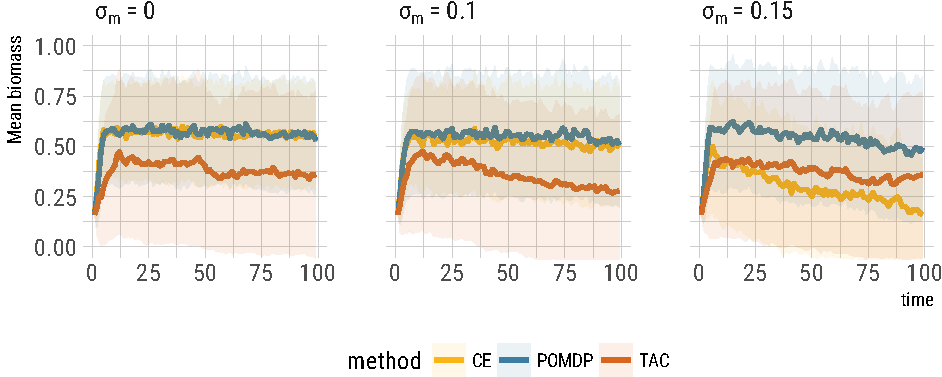
\includegraphics{manuscript_files/figure-latex/sims-1.pdf}
\caption{Average fish biomass under different management strategies
under increasing levels of measurement uncertainty. Each plot the mean
stock size over time across 100 replicate simulations under each policy:
constant escapement (CE), Total allowable catch (TAC = 80\% MSY), and
the proposed partially observed Markov decision process (POMDP) method.
Measurement error increases as a normal distribution with standard
deviation 0, 0.1, or 0.15, as indicated at the top of the panel.
Environmental stochasticity is fixed a standard deviation of 0.15 in
each panel. Carrying capacity K normalized to 1, r = 0.75. Additional
environmental noise levels and comparison to MSY rather than TAC can be
found in the supplementary material. \label{sims}}
\end{figure}

Figure \ref{sims} shows average fish biomass across 100 replicate
simulations under three different management strategies: constant
escapement (CE), total allowable catch (TAC; equal to 80\% MSY), and
partially observed Markov decision process (POMDP) management. Each
successive panel shows a subsequently higher level of measurement error,
from \(\sigma_m = 0\), \(\sigma_m = 0.1\), and \(\sigma_m = 0.15\), as
indicated. Standard deviation from the mean across replicate simulations
is shown as faint colored bands, indicating significant variation due to
stochasticity between individual replicates. In each panel shown in
Figure \ref{sims} stochastic recruitment (environmental noise) is set to
a moderate \(\sigma_g = 0.15\). In the absence of either environmental
noise or measurement error (Supplemental material, Figure S1) POMDP, CE,
and MSY would converge to stock at the \(B_{MSY}\), while TAC would
maintain the stock at a slightly higher level. The first panel of Figure
\ref{sims} shows that the the introduction of stochastic growth has a
significant negative impact on the TAC strategy (This impact is even
more severe for MSY, which always harvests strictly more than TAC by
definition, as, shown in Supplemental material Figure S2), which results
in an average biomass significantly lower than \(B_{MSY}\). Without
measurement error, the CE and POMDP strategies are nearly identical with
both approximately maintaining the stock at \(B_{MSY}\) despite the
significant environmental stochasticity. As measurement error increases
in the subsequent panels, CE and TAC strategies perform increasingly
poorly, while the POMDP continues to maintain the average stock close to
\(B_{MSY}\). Notably, CE is significantly more impacted by measurement
uncertainty than TAC, with CE averaging even lower biomass than TAC
under moderate measurement uncertainty.

Figure \ref{sims} confirms that the precautionary approach represented
by the TAC does indeed prove more robust to the problem of measurement
error than the optimization solution represented by CE. In general, we
expect that the rigid assumptions required of optimization will lead to
worse outcomes when those assumptions are not met than we see under the
corresponding heuristic approach. Yet it is important to bear in mind
that the opposite pattern was observed in the case of environmental
stochasticity, in which it was the heuristic TAC strategy rather than
the CE strategy that lead to the highest over-fishing rate. In contrast,
the POMDP approach successfully handles both stochasticity and
observation error, maintaining the stock near \(B_{MSY}\) levels that
produce the highest yield.

\begin{figure}
\centering
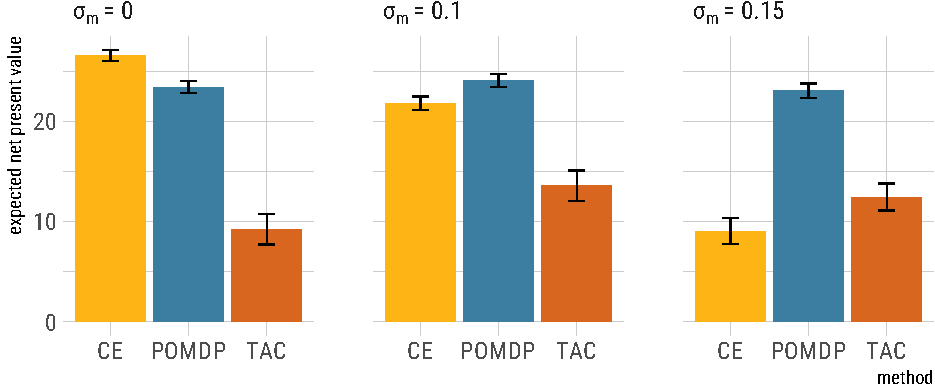
\includegraphics{manuscript_files/figure-latex/econ-1.pdf}
\caption{Expected net present value of the fishery across strategies
under increasing levels of measurement error \(\sigma_m\). Net present
value is th sum of all future harvests discounted over time and averaged
across 100 replicates simulations under each strategy, as shown in
Figure \ref{sims}. The value under constant escapement (CE) is optimal
when measurements are perfect but decreases rapidly with increasing
measurement error. The more cautious TAC is not economically optimal but
largely unimpacted by increasing error, while POMDP attains consistently
high economic yield despite the increasing uncertainty. \label{econ}}
\end{figure}

This pattern in management success in ecological terms (the relatively
recovery and maintenance of fish biomass) is also borne out in terms of
economic performance. Figure \ref{econ} shows the mean net present value
(averaging across replicates and discounting future profits by the
discount factor \(\gamma\)) for these same simulations at increasing
levels of measurement uncertainty. As before, environmental
stochasticity is set at \(\sigma_g = 0.15\). In the absence of
measurement uncertainty, constant escapement (CE) is optimal (as per
Reed (1979)), while the heuristic caution built into the total allowable
catch (TAC) strategy (at 80\% MSY) results in a sub-optimal economic
yield. The presence of stochasticity in recruitment
(\(\sigma_g = 0.15\)), also contributes to the reduction in yield under
TAC. Though CE is quite robust to the environmental stochasticity level,
this strategy proves very sensitive to increasing measurement error,
showing sharp declines in economic value, falling below the TAC economic
value at \(\sigma_m = 0.15\). Though the risk of stock collapse does
increase with increasing measurement error under TAC (as seen by the
mean declines in Figure \ref{sims}), these have little impact on the
economic value due to the discount rate. A smaller discount rate would
penalize unlikely but not improbable collapses more, since a significant
amount of time is required to realize those rare events. Supplemental
Figure S3 summarizes these economic trends across different noise values
\(\sigma_g\) and includes comparison to a simple MSY policy. In contrast
to the declining economic performance of CE and the consistently
sub-optimal economic yield for TAC, the POMDP strategy continues to
generate economic yields at approximately the optimal level (as attained
by CE in the absence of measurement error) despite the increasingly
uncertain measurements. This demonstrates that the reduced risk of stock
collapse and higher average stock biomass attained by the POMDP strategy
in the presence of high measurement error, Figure \ref{sims}) is not the
result of a trivial reduction in harvesting under all circumstances, but
rather, evidence of a more nuanced strategy that manages to account for
the uncertainty in measurement while maintaining a reasonable harvest.

\begin{figure}
\centering
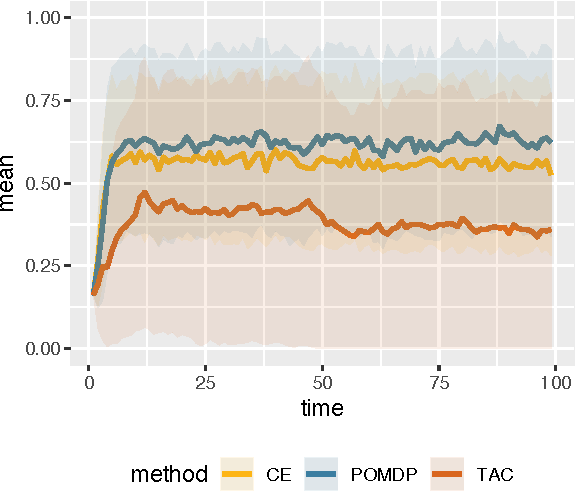
\includegraphics{manuscript_files/figure-latex/overest-1.pdf}
\caption{Average fish biomass when the POMDP strategy assumes a high
level of measurement uncertainty, while simulations reflect perfect
measurements. Despite this overestimation, biomass under POMDP strategy
closely tracks the optimal biomass under CE in the absence of
measurement error. \label{overest}}
\end{figure}

The POMDP strategy is also robust to overestimation of the level of
measurement uncertainty. In the simulation results shown in Figures
\ref{sims} and \ref{econ}, we have assumed that the level of measurement
uncertainty \(\sigma_m\) was known, and saw that ignoring this
uncertainty (as the CE policy does) has significant negative impact on
ecological and economic outcomes. If the level of measurement
uncertainty is not known precisely, \emph{overestimating} the
measurement error while using the POMDP strategy provides a
precautionary approach that can nevertheless achieve nearly optimal
ecological and economic outcomes. Figure \ref{overest} summarizes the
results of the same simulations as before, but under the scenario in
which the POMDP approach assumes a measurement error of
\(\sigma_m = 0.15\), when in fact all simulated measurements are made
without error (\(\sigma_m = 0\)). This represents an extreme case of
overestimating the measurement error. Stochastic growth remains the same
as before, \(\sigma_g = 0.15\), and simulations under TAC and CE
policies are shown for comparison. When measurement error is absent,
Reed's proofs hold and the CE strategy is optimal. Figure \ref{overest}
shows that the POMDP outcomes track almost exactly the CE outcomes
despite the misplaced assumption that measurements are quite poor. (As
we have already seen, the TAC strategy is insufficiently cautious for
this level of stochasticity in recruitment, resulting in
over-exploitation and long-term decline). The ability of the POMDP
solution to perform nearly optimally even when significantly
overestimating the level of measurement uncertainty contrasts sharply to
the significant declines from ignoring measurement uncertainty seen in
the CE solutions in Figure \ref{sims}. This demonstrates that while we
may not know precisely the level of measurement error, we achieve far
better outcomes overestimating measurement uncertainty than
underestimating it. This also underscores the observation that POMDP
policy is quite robust to the details of the uncertainty. We can get a
better understanding for the performance of POMDP in these simulations
by looking more closely at how any individual decision under a POMDP
strategy compares to the action chosen by the current alternatives.

\begin{figure}
\centering
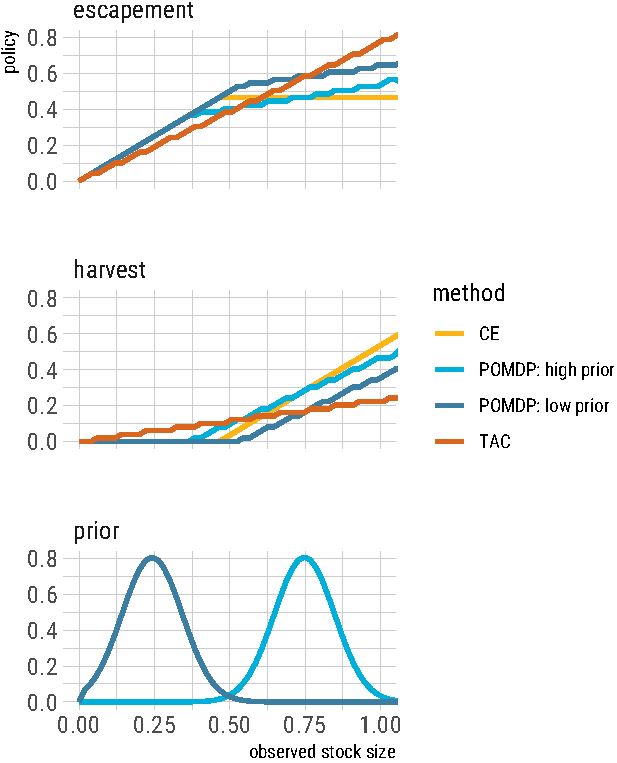
\includegraphics{manuscript_files/figure-latex/policy-1.pdf}
\caption{Comparison of the harvest and escapement policies under each
strategy as a function of the observed stock size. Escapement refers to
the expected fraction of fish left in the sea, \(x-h\), while harvest
refers to the target catch; two different conventions for plotting the
same action. Uniquely, the POMDP policy plot will depend not only on the
observed stock size, but also depends on prior information (bottom
panel) as determined from any prior observations and actions. Depending
on this prior it may harvest less or more than the other policies given
an identical observation.\label{policy}}
\end{figure}

To better understand the differences in performance of these strategies
and resolve the paradox of uncertainty, we must take a closer look at
how the specific action recommended by each policy compares given the
same observation. Figure \ref{policy} shows the action taken by each
strategy in response to a measurement of the stock size (biomass
estimate). These plots show, for any possible observations, which
strategy will attempt to harvest most and which will attempt to harvest
least. For comparison purposes, we plot policies both in terms of
expected escapement, \(S = Y - H\) as is typical in the optimal control
literature, (e.g. Reed 1979; Clark and Kirkwood 1986; Sethi et al.
2005), and also directly in terms of the harvest quota \(H\). These
plots clearly illustrate the contrast between the constant escapement
(CE) strategy and the precautionary Total Allowable Catch (TAC)
strategy: CE sets harvest strictly to zero for stocks estimated at
biomass below \(B_{MSY}\), while TAC permits a modest harvest of even
very small stocks. (Comparable plots with MSY can be found in the
Supplemental Material). In principle, the CE policy could depend on
\(\sigma_g\), but as Reed (1979) proved, the constant escapement level
with stochasticity is the same as in the deterministic case, S = D,
unless the noise level is quite high (comparison plots in Supplemental
material.) In contrast to this, our POMDP plots depend very much on both
the choice of \(\sigma_m\) and \(\sigma_g\). If \(\sigma_m = 0\), they
reduce exactly to the CE solution. Here we show the corresponding
policies for POMDP solutions focusing on \(\sigma_g = 0.15\) as above,
with a modest measurement uncertainty \(\sigma_m = 0.1\). Alternate
combinations of measurement uncertainty can be found in the appendix but
do not change the general pattern. In addition to an explicit dependence
on the measurement error, our POMDP solutions depend on another piece of
information: any prior observations of the stock size.

Differences in attention to prior beliefs,determined by prior
observations, drive the differences between the POMDP strategy and the
other strategies and can resolve the uncertainty paradox. While the
catch quota under both TAC and CE strategies can be completely
determined given the most recent observation of the stock size by using
the policy curves shown in Figure \ref{policy}, this is not the case for
the POMDP approach. This fundamental difference is key to understanding
the difference in performance and resolving the paradox of uncertainty.
The POMDP policy cannot be specified by the most recent observation
alone. Instead, the POMDP policy depends on all prior observations, not
just the most recent. The reason for this complexity comes from the
Markov property. Observations of the state in the perfectly observed
system satisfy the Markov property: once we have measured the current
biomass exactly, we cannot get any better estimate of the current stock
size by studying older measurements. When measurements are uncertain
this is no longer the case: intuitively, by comparing the most recent
measurement to previous observations we may be able to infer when any
given measurement is unusually high or unusually low. POMDP formalizes
this intuition by capturing the information from all previous
observations into a \emph{prior belief}. This prior belief is updated
after every subsequent action and observation in accordance with Bayes
Law. The mechanics of this process are well documented in the extensive
literature on POMDPs (e.g. Smallwood and Sondik 1973; Sondik 1978;
Kurniawati et al. 2008; Williams 2011), but for our purposes it is
sufficient to observe how this evolving prior belief serves to
continually adjust the POMDP policy. Supplemental Figure S9 (Appendix A)
illustrates how the prior belief evolves in response to subsequent
observations and actions over the course of an individual simulation.

Figure \ref{policy} shows two separate policy curves (in terms of
harvest and escapement) for the same POMDP solution given two different
prior belief distributions (panel 3, priors). While both priors shown
express considerable uncertainty about the precise stock size prior to
the most recent observation, the lower prior is centered at a value
\(\tfrac{1}{4}K\) stock size, while the high prior is centered at a
value of \(\tfrac{3}{4}K\), relative to a (post-harvest, before
observation) target size of \(B_{MSY} = K/2\). The POMDP policy is
determined by the combination of this prior information and the most
recent observation, as indicated by the two different POMDP curves for
harvest/escapement shown corresponding to the different priors. As with
the other policies, the higher the most recent observation (x axis) the
higher the POMDP recommended harvest. Yet unlike the alternative
strategies, the POMDP solution always reflects the prior information.
Consequently, relative to constant escapement (that is, no measurement
error), the POMDP with low prior starts harvesting only at higher stock
sizes and always harvests less. In contrast under the high prior, the
POMDP always harvests at the same or higher level than the constant
escapement solution.

\textbf{A resolution to the paradox.}

Herein lies our resolution to the paradox of uncertainty. Previous work
created this paradox by suggesting that increased harvest rates
(decreased target escapement) would often be the rational response to
increased uncertainty. The exact solutions from the POMDP reveal that
this is only an accident of the assumptions: it is indeed true that
under certain circumstances, harvest levels should increase relative to
the case of no uncertainty, but \emph{only when prior knowledge suggests
the stock size should be much higher than the most recent estimate would
suggest}. In the POMDP solution, all information must be put into its
historical (and constantly updated) context. When a measurement roughly
matches the expectation of this prior context, Figure \ref{policy} shows
that the optimal response from POMDP is roughly comparable or slightly
more cautious to the harvest under no uncertainty, and not more
aggressive as the paradox would suggest. Measurements that exceed
expectations are tempered with some skepticism: while the CE solution is
willing to meet a high stock measurement with a large harvest, the POMDP
solutions increase harvest more cautiously.

This difference between underestimating and overestimating accounts for
the poor performance of the CE solution under large measurement
uncertainty, where it over-harvests whenever measurements are too large.
Even though underestimating is equally likely under the measurement
uncertainty model, sooner or later a run of ``heads'', a sequence of
overestimations relative to the true stock, can drive stocks to very low
levels where the chance of local extinction becomes possible. It is
precisely this asymmetry: that too much over-harvesting leads to an
irreversible state of extinction, while too much under-harvesting is
always reversible (modulo some lost revenue) that lay behind Clark's
original intuition that there was something fishy about Reed's result
that \(S = D\): that uncertainty required no extra caution. Constant
escapement is particularly susceptible to over-harvesting starting from
stock sizes much higher than \(B_{MSY}\) since its bang-bang optimal
solution attempts to bring stocks back to target level as fast as
possible. CE is not so vulnerable to collapse from small stock sizes,
since it shuts down all harvests once estimates fall below \(B_{MSY}\).
Stock collapse under TAC can also be driven by such a string of heads,
but is unlikely at high stock sizes since harvest never exceeds
\(H_{MSY}\). In both cases, some measurement uncertainty interacts with
inherent stochasticity, which provides a continued source of variation
to sizes above \(B_{MSY}\), where CE strategy is most vulnerable, and
below \(B_{MSY}\), where TAC is most vulnerable.

\begin{figure}
\centering
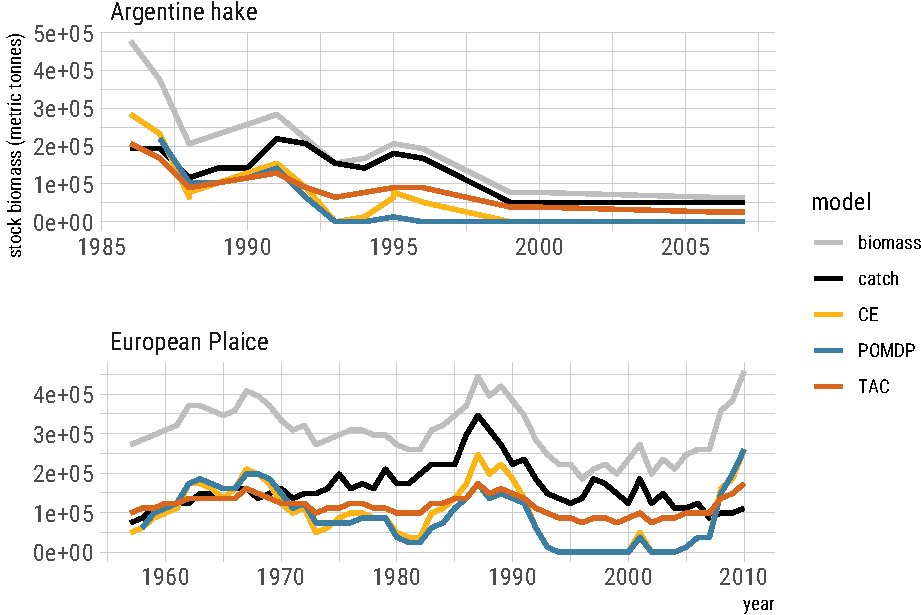
\includegraphics{manuscript_files/figure-latex/historical-1.pdf}
\caption{Comparisons of harvest level that would be recommended by
policies considered here relative to historical harvest levels in two
commercial fish stocks. POMDP solution assumes a measurement error of
10\%. \label{historical}}
\end{figure}

\textbf{Historical examples and implementation}.

So far we have focused on simulation and an examination of the relative
policies under different prior information. Figure \ref{historical}
compares the harvest level that would have been recommended by each of
the strategies we have considered here against the historically observed
catch recorded for two commercially fished stocks: Argentine Hake and
European Plaice. Historical estimates of biomass and catch are taken
from the R.A. Myers Legacy Stock Assessment database (Ricard et al.
2011). Posterior distributions for parameters for the Gordon-Schaefer
model are estimated with uncertainty through Markov Chain Monte Carlo
using \texttt{nimble} (de Valpine et al. 2017) on the historical data,
illustrating how this process might be done in more complex models as
well (details and code in Supplement, Appendix B). \(B_{MSY}\) and
corresponding TAC and CE policies are calculated based on posterior mean
estimates of the model parameters, along with POMDP solution assuming a
10\% measurement error rate. Though measurement error could be estimated
directly from the raw data, this would not reflect the true measurement
uncertainty arising from the stock assessment process. Each strategy is
then compared to historical observations to determine a recommended
harvest. As we have seen, the TAC and CE harvest policies are uniquely
determined by the observed stock size relative to \(B_{MSY}\), but the
POMDP policy must be re-calculated each time step to reflect both the
prior observation and prior action.

These historical examples provide another useful lens to compare how the
different strategies respond in the face of fluctuations in real data,
rather than model simulations. In both stocks, historical catch almost
always exceeds that recommended by any of our strategies, falling closer
to the MSY value estimated (see Appendix B). In Argentine Hake, the
persistent declines result in both POMDP and CE strategies quickly
closing down the fishery in an attempt to let the stock recover to a
more productive target biomass, while TAC persists with merely a reduced
harvest. A small recovery of biomass in 1995 is met by an immediate
uptick in harvest under CE, while the POMDP response is more
conservative. The example of European Plaice illustrates more volatility
in the stock size, revealing further differences in the strategies.
Despite this volatility, the TAC level remains relatively level across
all five decades, rising or dipping only slightly with changes in stock
size. In contrast, the CE harvest tracks this volatility almost exactly.
Here, the POMDP solution falls in between these extremes, almost
mirroring which-ever of the two policies is more conservative: the POMDP
solution matches the dips in harvest taken by CE to allow the stock to
recover most quickly, but does not track the doubling of harvests
recommended by CE in the mid 1980, increasingly only to the more modest
harvest recommended by the TAC policy. Once again, we see that POMDP
solution provides a more consistently precautionary policy than either
the over-simplified optimal control solution of CE or the more
rule-of-thumb approach represented by TAC. Though we have seen that the
POMDP solution need not always be more conservative (lower harvest) than
these strategies, it makes use of the all prior observations to tune the
level of caution appropriately.

\section{Discussion}\label{discussion}

Using modern algorithms we have been able to crack the nut of
measurement uncertainty in the optimal management of marine fisheries
and debunk long-standing paradoxes that increased measurement
uncertainty should be met with larger harvests. We have demonstrated
that both existing optimal control approaches and existing precautionary
approaches result in over-exploitation and long term declines of fish
stocks, as well as reduced economic value, while in contrast, the POMDP
approach is able to deliver both ecological and economic recovery
despite uncertainty in measurements. These results have important
implications for both global fisheries and ecological management more
generally. In marine fisheries, evidence of such over-exploitation has
already been well documented (Worm et al. 2006, 2009; Costello et al.
2016). Our results suggest that measurement uncertainty may contribute
to this pattern, as such errors lead to over-exploitation under current
best practices such as MSY, TAC or CE, which have previously been
thought to be sufficient to ensure the recovery of stocks world-wide
(Costello et al. 2016).

Our results also have important consequences for ecological management
more generally. The study and application of management strategies such
as MSY and CE underpin much of conservation and natural resource
management in forest management and many other terrestrial ecosystems
(e.g. Clark and Mangel 2000). Descision making under uncertainty is a
central challenge for ecology and conservation biology (Polasky et al.
2011), which we have long attempted to address through either simplified
optimal control models or more heuristic approaches such as the
precautionary principle and resilience thinking (Fischer et al. 2009).
We have illustrated how both of these approaches can fail to provide an
adequate strategy when faced with measurement uncertainty. To avoid this
pitfall, a strategy must be dynamic to make best use of the available
information without assuming that information is perfect. The
simplisitic optimal control approach of CE fails by placing too much
confidence in measurements even when they are significantly at odds with
prior expectations. Similarly, the TAC approach also fails due to it's
reliance on a simple one-size-fits-all strategy, not reducing catch
quotas sufficiently when stocks are too low but also failing to increase
them when stocks are higher. It is precisely this ability to adapt the
policy in response to available information, as illustrated in Figure
\ref{policy}, that makes the POMDP approach successful. Nevertheless, it
may be tempting to see these results as either trivial or impractical,
but a closer inspection reveals they are neither.

First, it may seem obvious that POMDP would out-preform more primitive
optimal control solutions such as CE, but this was hardly a forgone
conclusion. Indeed, the previous example of Reed (1979) had proven that
the complex stochastic dynamic programming solutions required to
accommodate stochastic dynamics would perform no better than the simple
maximization based purely on the deterministic model. If stochasticity
doesn't matter, it is easy to believe that measurement error would be
minor at best. In fact, we find that once we account for measurement
error, the effects of both stochasticity and measurement have a
significant influence over the optimal policy. It is similarly tempting
to dismiss the better performance of POMDP against a more
rule-of-thumb{[}\^{}1{]} based strategy like the TAC scenario considered
here (fishing at 80\% MSY), but once again this was not a forgone
conclusion. While a better economic return might reasonably be expected
of the optimization approach, it was not obvious that POMDP would also
be at times more cautious than the rule of thumb, able to deliver both
higher economic returns by harvesting more when it was safe to do so,
and higher ecological recovery by harvesting even less than TAC when
necessary. These results highlight the difficulty of finding effective
heuristic rules and underscore the power and utility of more
sophisticated strategies such as POMDP which can make the best use of
all available information.

\^{}1: Given the sophisticated policies often in place to determine
actual TAC levels, one might object to our characterization of this as
merely a rule-of-thumb. We use this term merely to distinguish it from
the optimal control approach -- that despite technical precision, TAC
adjustments are set by a heuristic instead of the result of some dynamic
optimization algorithm as in CE and POMDP.

Second, we must ask if the policies derived from POMDP are practical. As
with constant escapement, the POMDP solutions we considered here result
in more year-to-year variation in harvest, and include the possibility
of fishing moratorium to allow stocks to recover -- decisions that many
view as economically or socially unacceptable. While resolving this
debate is beyond the scope of this paper, a few observations are
relevant: (A) Stocks already managed under constant escapement, such as
US salmon fisheries, are already subject to the possibility of these
moratoriums. (B) It is straight-forward to introduce constraints on the
minimal acceptable harvest level and/or include the additional costs of
closing a fishery in the utility function optimized by POMDP. (C)
Fisheries today are not managed at either their maximum ecological or
economic potential. Taken as a whole, most ocean fisheries yield a net
negative economic return (World Bank and FAO 2009), with fishing
persisting only with the support of government subsidies (Arnason 2012),
meanwhile some 68\% of global fisheries are in poor biological condition
(Costello et al. 2016). While the causes for this are both complex and
numerous, we have seen that both the economic inefficiency and
ecological health suffer under TAC/MSY and CE based management. Arnason
(2012) and Costello et al. (2016) have both argued that a rights-based
approach to fisheries management (RBFM) would lead to self adoption of
precisely such optimal policies.

Third: are the examples considered here too simple? The strategies we
have compared against underpin both current practice and management
aspirations. Together, MSY and TAC-based management reflects much of
modern best practice as it is understood in fisheries management and
elsewhere. While real-world application of these approaches frequently
involves more complex models, the models we have considered here are the
very ones under which these strategies were designed and tested, and
there is little reason to believe they would perform better under more
complex cases such as age-structured models that do not always meet
those assumptions (e.g. Holden and Conrad 2015). The relatively poor
ecological and economic performance of these common best-practices
relative to the alternative approach of POMDP is thus reason enough for
concern. This issue is further underscored by the reality of both
long-running ecological deterioration (Worm et al. 2006, 2009) and
economic costs of global fisheries.

Fourth: is the approach taken here too complex to be feasible? The
importance of simple and effective rules of thumb in conservation
management has been well documented (e.g. Chadès et al. 2011).
Sophisticated and computationally intensive approaches such as POMDP may
seem improbable at a time when many areas of natural resource
management, even simple, rule-of-thumb based methods struggle to take
root. And yet, in this same age we rely on far more complex and
computationally intensive algorithms to perform far more trivial tasks
such as determining what advertisements we see. Surely a planet that can
afford such complex optimization for how advertising space is allocated
on a small screen can one day manage it's natural resources and
conservation efforts with such tools?

\subsection{Future directions}\label{future-directions}

Several limitations that have been studied in fully observed (MDP)
optimal decision problems, such as parameter uncertainty (e.g. Ludwig
and Walters 1982), model uncertainty (Williams 2001; Boettiger et al.
2015) and adaptive management (e.g. Walters and Hilborn 1976) remain
largely open challenges for partially observed systems. Future work
could extend this analysis to more complex models, such as those with
age structure, as (Holden and Conrad 2015) does for the fully observed
case. Another limiting assumption common to MDPs and POMDPs is that of
stationary dynamics: that the population dynamics equation itself is not
changing over time. In reality, forces such as climate change and other
forms of environmental variations violate this assumption (Britten et
al. 2017). Direct approaches such as Fackler and Pacifici (2014)'s
adaptation of Mixed Observability MDP (Ong et al. 2010) do not scale to
the number of states and actions considered here. A value of information
(VOI) analysis for POMDP (e.g. Johnson and Williams 2015; Memarzadeh and
Pozzi 2016), could identify when it is worthwhile to actively reduce
measurement error.

\section*{References}\label{references}
\addcontentsline{toc}{section}{References}

\hypertarget{refs}{}
\hypertarget{ref-Arnason2012}{}
Arnason, R. 2012. Property rights in fisheries: How much can individual
transferable quotas accomplish? Review of Environmental Economics and
Policy 6:217--236.

\hypertarget{ref-Beverton1957}{}
Beverton, R., and S. Holt. 1957. On the Dynamics of Exploited Fish
Populations. Chapman; Hall, London.

\hypertarget{ref-Boettiger2015}{}
Boettiger, C., M. Mangel, and S. Munch. 2015. Avoiding tipping points in
fisheries management through Gaussian process dynamic programming.
Proceedings of the Royal Society B: Biological Sciences
282:20141631--20141631.

\hypertarget{ref-sarsop-pkg}{}
Boettiger, C., J. Ooms, and M. Memarzadeh. 2018. Sarsop: Approximate
pomdp planning software.

\hypertarget{ref-Botsford1997}{}
Botsford, L. W., J. C. Castilla, and C. Peterson. 1997. The management
of fisheries and marine ecosystems. Science 277:509--515.

\hypertarget{ref-Britten2017}{}
Britten, G., M. Dowd, L. Kanary, and B. Worm. 2017. Extended fisheries
recovery timelines in a changing environment. Nature Communications.

\hypertarget{ref-Chades2011}{}
Chadès, I., T. G. Martin, S. Nicol, M. A. Burgman, H. P. Possingham, and
Y. M. Buckley. 2011. General rules for managing and surveying networks
of pests, diseases, and endangered species. Proceedings of the National
Academy of Sciences 108:8323--8.

\hypertarget{ref-Chades2008}{}
Chadès, I., E. McDonald-Madden, M. a McCarthy, B. Wintle, M. Linkie, and
H. P. Possingham. 2008. When to stop managing or surveying cryptic
threatened species. Proceedings of the National Academy of Sciences
105:13936--40.

\hypertarget{ref-Clark1973}{}
Clark, C. W. 1973. Profit maximization and the extinction of animal
species. Journal of Political Economy 81:950--961.

\hypertarget{ref-Clark1990}{}
Clark, C. W. 1990. Mathematical Bioeconomics: The Optimal Management of
Renewable Resources, 2nd Edition. Wiley-Interscience.

\hypertarget{ref-Clark1986}{}
Clark, C. W., and G. P. Kirkwood. 1986. On uncertain renewable resource
stocks: Optimal harvest policies and the value of stock surveys. Journal
of Environmental Economics and Management 13:235--244.

\hypertarget{ref-Clark2000}{}
Clark, C. W., and M. Mangel. 2000. Dynamic state variable models in
ecology. Oxford University Press, Oxford.

\hypertarget{ref-Costello2016}{}
Costello, C., D. Ovando, T. Clavelle, C. K. Strauss, R. Hilborn, M. C.
Melnychuk, T. A. Branch, et al. 2016. Global fishery prospects under
contrasting management regimes. Proceedings of the National Academy of
Sciences 113:5125--5129.

\hypertarget{ref-nimble}{}
de Valpine, P., D. Turek, C. J. Paciorek, C. Anderson-Bergman, T.
Duncan, and R. Bodik. 2017. Programming With Models: Writing Statistical
Algorithms for General Model Structures With NIMBLE. Journal of
Computational and Graphical Statistics 26:403--413.

\hypertarget{ref-Dichmont2016}{}
Dichmont, C. M., R. A. Deng, A. E. Punt, J. Brodziak, Y.-J. Chang, J. M.
Cope, J. N. Ianelli, et al. 2016. A review of stock assessment packages
in the united states. Fisheries Research 183:447--460.

\hypertarget{ref-Engen1997}{}
Engen, S., R. Lande, and B. Sæther. 1997. Harvesting strategies for
fluctuating populations based on uncertain population estimates. Journal
of Theoretical Biology 186:201--212.

\hypertarget{ref-Fackler2014b}{}
Fackler, P., and R. Haight. 2014. Monitoring as a partially observable
decision problem. Resource and Energy Economics 37:226--241.

\hypertarget{ref-Fackler2014}{}
Fackler, P., and K. Pacifici. 2014. Addressing structural and
observational uncertainty in resource management. Environmental
Management 133:27--36.

\hypertarget{ref-Fischer2009}{}
Fischer, J., G. D. Peterson, T. a Gardner, L. J. Gordon, I. Fazey, T.
Elmqvist, A. Felton, et al. 2009. Integrating resilience thinking and
optimisation for conservation. Trends in ecology \& evolution
24:549--54.

\hypertarget{ref-Gordon1954}{}
Gordon, H. S., and C. Press. 1954. The Economic Theory of a
Common-Property Resource: The Fishery. Journal of Political Economy
62:124--142.

\hypertarget{ref-Hilborn2010}{}
Hilborn, R. 2010. Pretty Good Yield and exploited fishes. Marine Policy
34:193--196.

\hypertarget{ref-Holden2015}{}
Holden, M., and J. Conrad. 2015. Optimal escapement in stage-structured
fisheries with environmental stochasticity. Mathematical biosciences
269:76--85.

\hypertarget{ref-Holling1973}{}
Holling, C. S. 1973. Resilience and Stability of Ecological Systems.
Annual Review of Ecology and Systematics 4:1--23.

\hypertarget{ref-Johnson2015}{}
Johnson, F. A., and B. K. Williams. 2015. A Decision-Analytic Approach
to Adaptive Resource Management. Pages 61--84 \emph{in} C. R. Allen and
A. S. Garmestani, eds. Adaptive management of social-ecological systems.
Springer Netherlands, Dordrecht.

\hypertarget{ref-Kaelbling1998}{}
Kaelbling, L. P., M. L. Littman, and A. R. Cassandra. 1998. Planning and
Acting in Partially Observable Stochastic Domains. Artificial
Intelligence 101:99--134.

\hypertarget{ref-Kurniawati2008}{}
Kurniawati, H., D. Hsu, and W. S. Lee. 2008. SARSOP : Efficient
Point-Based POMDP Planning by Approximating Optimally Reachable Belief
Spaces. Proceedings of Robotics: Science and Systems IV.

\hypertarget{ref-Larkin1977}{}
Larkin, P. a. 1977. An Epitaph for the Concept of Maximum Sustained
Yield. Transactions of the American Fisheries Society 106:1--11.

\hypertarget{ref-Levin2008}{}
Levin, S. A., and J. Lubchenco. 2008. Resilience, Robustness, and Marine
Ecosystem-based Management. BioScience 58:27--32.

\hypertarget{ref-Ludwig1981}{}
Ludwig, D., and C. Walters. 1981. Measurement errors and uncertainty in
parameter estimates for stock and recruitment. Journal of Canadian
Fisheries and Aquatic Sciences 38:711--720.

\hypertarget{ref-Ludwig1982}{}
Ludwig, D., and C. J. Walters. 1982. Optimal harvesting with imprecise
parameter estimates. Ecological Modelling 14:273--292.

\hypertarget{ref-Mace2001}{}
Mace, P. M. 2001. A new role for MSY in single-species and
ecosystem\(\backslash\)rapproaches to fisheries stock assessment and
management. Fish and Fisheries 2:2--32.

\hypertarget{ref-Mangel1988}{}
Mangel, M., and C. W. Clark. 1988. Dynamic Modeling in Behavioral
Ecology. (J. Krebs \& T. Clutton-Brock, eds.). Princeton University
Press, Princeton.

\hypertarget{ref-Marescot2013}{}
Marescot, L., G. Chapron, I. Chadès, P. L. Fackler, C. Duchamp, E.
Marboutin, and O. Gimenez. 2013. Complex decisions made simple: a primer
on stochastic dynamic programming. Methods in Ecology and Evolution
n/a--n/a.

\hypertarget{ref-May1977}{}
May, R. M. 1977. Thresholds and breakpoints in ecosystems with a
multiplicity of stable states. Nature 269:471--477.

\hypertarget{ref-Memarzadeh2016b}{}
Memarzadeh, M., and M. Pozzi. 2016. Value of information in sequential
decision making: component inspection, permanent monitoring and
system-level scheduling. Reliability Engineering \& System Safety
154:137--151.

\hypertarget{ref-Moxnes2003}{}
Moxnes, E. 2003. Uncertain measurements of renewable resources:
approximations, harvesting policies and value of accuracy. Journal of
Environmental Economics and Management 45:85--108.

\hypertarget{ref-Ong2010}{}
Ong, S., S. Png, D. Hsu, and W. Lee. 2010. Planning under uncertainty
for robotic tasks with mixed observability. The International Journal of
Robotics Research 29:1053--1068.

\hypertarget{ref-Petchy2015}{}
Petchey, O. L., M. Pontarp, T. M. Massie, S. Kéfi, A. Ozgul, M.
Weilenmann, G. M. Palamara, et al. 2015. The ecological forecast
horizon, and examples of its uses and determinants. Ecology Letters
18:597--611.

\hypertarget{ref-Pineau2003}{}
Pineau, J., G. Gordon, and S. Thrun. 2003. Point-based value iteration:
An anytime algorithm for POMDPs. IJCAI International Joint Conference on
Artificial Intelligence 1025--1030.

\hypertarget{ref-Polasky2011}{}
Polasky, S., S. R. Carpenter, C. Folke, and B. Keeler. 2011.
Decision-making under great uncertainty: environmental management in an
era of global change. Trends in ecology \& evolution 1--7.

\hypertarget{ref-Reed1979}{}
Reed, W. J. 1979. Optimal escapement levels in stochastic and
deterministic harvesting models. Journal of Environmental Economics and
Management 6:350--363.

\hypertarget{ref-RAM}{}
Ricard, D., C. Minto, O. Jensen, and J. Baum. 2011. Examining the
knowledge base and status of commercially exploited marine species with
the RAM Legacy Stock Assessment Database. Fish and Fisheries
13:380--398.

\hypertarget{ref-Roughgarden1996}{}
Roughgarden, J. E., and F. Smith. 1996. Why fisheries collapse and what
to do about it. Proceedings of the National Academy of Sciences 93:5078.

\hypertarget{ref-Schaefer1954}{}
Schaefer, M. B. 1954. Some aspects of the dynamics of populations
important to the management of the commercial marine fisheries. Bulletin
of the Inter-American Tropical Tuna Commission 1:27--56.

\hypertarget{ref-Sethi2005}{}
Sethi, G., C. Costello, A. Fisher, M. Hanemann, and L. Karp. 2005.
Fishery management under multiple uncertainty. Journal of Environmental
Economics and Management 50:300--318.

\hypertarget{ref-Smallwood1973}{}
Smallwood, R. D., and E. J. Sondik. 1973. The Optimal Control of
Partially Observable Markov Decision Processes over a Finite Horizon.

\hypertarget{ref-Sondik1978}{}
Sondik, E. J. 1978. The Optimal Control of Partially Observable Markov
Processes Over the Infinite Horizon : Discounted Costs. Operations
Research 26:282--304.

\hypertarget{ref-Walters1976}{}
Walters, C. J., and R. Hilborn. 1976. Adaptive Control of Fishing
Systems. Journal of the Fisheries Research Board of Canada 33:145--159.

\hypertarget{ref-Walters1978}{}
---------. 1978. Ecological Optimization and Adaptive Management. Annual
Review of Ecology and Systematics 9:157--188.

\hypertarget{ref-Williams2001}{}
Williams, B. K. 2001. Uncertainty , learning , and the optimal
management of wildlife. Environmental and Ecological Statistics
8:269--288.

\hypertarget{ref-Williams2011}{}
---------. 2011. Resolving structural uncertainty in natural resources
management using POMDP approaches. Ecological Modelling 222:1092--1102.

\hypertarget{ref-FAO2009}{}
World Bank and FAO. 2009. The Sunken Billions. The Economic
Justification for Fisheries Reform.

\hypertarget{ref-Worm2006}{}
Worm, B., E. B. Barbier, N. Beaumont, J. E. Duffy, C. Folke, B. S.
Halpern, J. B. C. Jackson, et al. 2006. Impacts of biodiversity loss on
ocean ecosystem services. Science (New York, N.Y.) 314:787--90.

\hypertarget{ref-Worm2009}{}
Worm, B., R. Hilborn, J. K. Baum, T. A. Branch, J. S. Collie, C.
Costello, M. J. Fogarty, et al. 2009. Rebuilding global fisheries.
Science (New York, N.Y.) 325:578--85.

\end{document}


